\documentclass[12pt,a4paper]{article}

\usepackage[utf8]{inputenc}
\usepackage[T5]{fontenc}
\usepackage[vietnamese]{babel}
\usepackage{geometry}
\usepackage{graphicx}
\usepackage{float}
\usepackage{array}
\usepackage{longtable}
\usepackage{hyperref}
\usepackage{verbatim}

\geometry{
    left=3cm,
    right=2cm,
    top=2.5cm,
    bottom=2.5cm
}

\renewcommand{\arraystretch}{1.3}
\setlength{\parindent}{1cm}
\setlength{\parskip}{6pt}

\newcommand{\demoimage}[3]{
    \begin{figure}[H]
        \centering
        \IfFileExists{#1}{
            \includegraphics[width=0.85\textwidth]{#1}
        }{
            \fbox{
                \begin{minipage}[c][5cm][c]{0.85\textwidth}
                    \centering
                    Chua co anh: \texttt{#1}\\
                    #2
                \end{minipage}
            }
        }
        \caption{#3}
    \end{figure}
}

\newcommand{\umldiagram}[3]{
    \subsection{#2}
    \IfFileExists{#1.png}{
        \begin{figure}[H]
            \centering
            \includegraphics[width=0.95\textwidth]{#1.png}
            \caption{#3}
        \end{figure}
    }{
        Chua co file anh \texttt{#1.png}. Duoi day la code PlantUML dung de tao bieu do:
        \verbatiminput{#1.puml}
    }
}

\begin{document}

% ================= TRANG BIA =================
\begin{titlepage}
    \centering

    {\Large TRUONG DAI HOC ...}\\
    {\Large KHOA ...}\\[2cm]

    {\LARGE \textbf{BAO CAO BAI TAP LON}}\\[0.5cm]
    {\Large \textbf{MON: LAP TRINH HUONG DOI TUONG}}\\[1.5cm]

    {\Huge \textbf{WILD-LIFE ECO SIMULATION}}\\[0.5cm]
    {\Large \textbf{He thong mo phong he sinh thai hoang da}}\\[2cm]

    \begin{flushleft}
        \textbf{Giang vien huong dan:} ...\\
        \textbf{Nhom thuc hien:} ...\\
        \textbf{Lop:} ...\\
    \end{flushleft}

    \vspace{1cm}

    \begin{tabular}{|c|l|c|}
        \hline
        \textbf{STT} & \textbf{Ho va ten} & \textbf{MSSV} \\
        \hline
        1 & TungTran / TungSoYeu & ... \\
        \hline
        2 & davidtaiduc & ... \\
        \hline
        3 & Thanh vien khac neu co & ... \\
        \hline
    \end{tabular}

    \vfill

    {\large TP. Ho Chi Minh, thang 06 nam 2026}
\end{titlepage}

\tableofcontents
\newpage

% ================= NOI DUNG =================

\section{Gioi thieu de tai}

De tai \textbf{Wild-Life Eco Simulation} la mot ung dung JavaFX mo phong he sinh thai hoang da theo huong lap trinh huong doi tuong. Chuong trinh mo phong ban do gom dong co, rung ram, ho nuoc, bun, vach da va bui ram. Tren ban do co nhieu loai thuc the nhu co, cay an qua, tho, huou, soi, ho, voi, tho san, ca va vit.

Muc tieu cua chuong trinh la mo phong hanh vi sinh ton cua cac loai sinh vat trong moi truong thay doi theo mua. Moi dong vat co trang thai suc khoe, do doi, do khat, toc do, tam nhin va chien luoc hanh vi rieng. Nguoi dung co the bat dau hoac tam dung mo phong, dieu chinh toc do, doi che do hien thi, them thuc the va quan sat thong ke trong qua trinh chay.

\section{Phan cong cong viec cac thanh vien trong nhom}

Thong tin thanh vien duoc dien dua tren lich su Git cua project. Neu nhom co ten that hoac MSSV khac, co the cap nhat truc tiep trong bang sau.

\begin{table}[H]
    \centering
    \caption{Phan cong cong viec va ti le dong gop}
    \begin{tabular}{|c|p{4cm}|p{7cm}|c|}
        \hline
        \textbf{STT} & \textbf{Thanh vien} & \textbf{Cong viec phu trach} & \textbf{Dong gop} \\
        \hline
        1 & TungTran / TungSoYeu
        & Xay dung cau truc Maven, thiet ke cac package chinh, phat trien engine mo phong, model entity, logic mua, sinh san, va cap nhat README.
        & 55\% \\
        \hline
        2 & davidtaiduc
        & Ho tro phat trien tinh nang, chinh sua va tich hop mot phan logic chuong trinh theo lich su commit.
        & 20\% \\
        \hline
        3 & Thanh vien khac neu co
        & Ho tro kiem thu, ve UML, chuan bi bao cao, anh demo va thuyet trinh.
        & 25\% \\
        \hline
    \end{tabular}
\end{table}

\subsection{Mo ta dong gop cu the}

\begin{itemize}
    \item \textbf{Phan thiet ke va kien truc:} xay dung kien truc tach biet Model, View, Engine, Strategy, Sound va Util.
    \item \textbf{Phan lap trinh chinh:} cai dat cac lop \texttt{Entity}, \texttt{Animal}, \texttt{Plant}, cac loai dong vat, cac loai thuc vat, \texttt{SimulationEngine}, \texttt{EntityManager}, \texttt{WorldMap}.
    \item \textbf{Phan giao dien:} xay dung \texttt{GameView}, \texttt{Renderer}, \texttt{BasicRenderer}, \texttt{SpriteRenderer}, camera, thanh dieu khien va bang thong ke.
    \item \textbf{Phan kiem thu:} viet test JUnit cho hanh vi san moi, doi strategy khi doi, sat thuong phuc kich cua ho va kha nang an nap trong bui ram.
\end{itemize}

\section{Chi tiet nhat ky lam viec nhom}

\begin{longtable}{|c|c|p{4cm}|p{6cm}|p{3cm}|}
    \hline
    \textbf{STT} & \textbf{Thoi gian} & \textbf{Thanh vien} & \textbf{Noi dung cong viec} & \textbf{Ket qua} \\
    \hline
    1 & Giai doan 1 & Ca nhom & Chon de tai mo phong he sinh thai, xac dinh doi tuong mo phong va cac yeu cau OOP can the hien. & Thong nhat de tai Wild-Life Eco Simulation. \\
    \hline
    2 & Giai doan 2 & TungTran / TungSoYeu & Khoi tao project Java Maven, cau hinh Java 21, JavaFX, JUnit, Maven Wrapper va module \texttt{com.ecosim}. & Project co the build va chay bang \texttt{mvnw.cmd}. \\
    \hline
    3 & Giai doan 3 & Ca nhom & Thiet ke cac package \texttt{model}, \texttt{engine}, \texttt{strategy}, \texttt{view}, \texttt{sound}, \texttt{util}. & Co cau truc package ro rang, tach biet trach nhiem. \\
    \hline
    4 & Giai doan 4 & TungTran / TungSoYeu & Cai dat he thong thuc the gom \texttt{Entity}, \texttt{Animal}, \texttt{Plant}, cac loai dong vat va thuc vat. & Hoan thanh mo hinh lop chinh cua he sinh thai. \\
    \hline
    5 & Giai doan 5 & Ca nhom & Cai dat \texttt{SimulationEngine}, \texttt{EntityManager}, ban do, mua, sinh san, di chuyen va xu ly va cham. & Mo phong co the chay theo tick va thay doi theo mua. \\
    \hline
    6 & Giai doan 6 & Ca nhom & Cai dat Strategy Pattern cho hanh vi sinh ton: thu dong, so hai, san moi, lieu linh. & Dong vat co hanh vi linh hoat va co the doi strategy khi runtime. \\
    \hline
    7 & Giai doan 7 & Ca nhom & Xay dung giao dien JavaFX, canvas, camera, renderer, sprite, am thanh va bang thong ke. & Nguoi dung co the tuong tac voi mo phong. \\
    \hline
    8 & Giai doan 8 & Ca nhom & Viet test, sua loi va hoan thien README, huong dan chay, chuan bi bao cao. & Co test JUnit va tai lieu huong dan su dung. \\
    \hline
\end{longtable}

\section{Thong ke du lieu thu thap duoc}

De tai nay khong thu thap du lieu khao sat ben ngoai ma su dung du lieu cau hinh va du lieu mo phong duoc khoi tao trong chuong trinh. Bang duoi day thong ke cac tap du lieu chinh ma he thong su dung khi chay.

\begin{table}[H]
    \centering
    \caption{Thong ke du lieu mo phong}
    \begin{tabular}{|c|p{5cm}|c|p{5cm}|}
        \hline
        \textbf{STT} & \textbf{Loai du lieu} & \textbf{So luong} & \textbf{Nguon du lieu} \\
        \hline
        1 & Kich thuoc ban do & 120 x 80 = 9600 tile & \texttt{Constants.MAP\_WIDTH}, \texttt{Constants.MAP\_HEIGHT} \\
        \hline
        2 & Loai dia hinh & 6 & \texttt{TerrainType}: dong co, rung ram, ho nuoc, bun, vach da, bui ram \\
        \hline
        3 & Mua trong nam & 4 & \texttt{Season}: xuan, ha, thu, dong \\
        \hline
        4 & Thuc vat khoi tao ban dau & 150 & 120 co, 30 cay an qua trong \texttt{EntityManager.spawnInitialEntities()} \\
        \hline
        5 & Dong vat khoi tao ban dau & 78 & Tho, huou, soi, ho, voi, tho san, ca, vit \\
        \hline
        6 & Tong thuc the ban dau & 228 & Tong so thuc vat va dong vat khi bat dau mo phong \\
        \hline
        7 & Anh sprite PNG & 9 & Thu muc \texttt{src/main/resources/sprites} \\
        \hline
        8 & Tep am thanh WAV & 6 & Thu muc \texttt{src/main/resources/sounds} \\
        \hline
        9 & Test case JUnit & 5 & Cac file test trong \texttt{src/test/java} \\
        \hline
    \end{tabular}
\end{table}

\begin{table}[H]
    \centering
    \caption{So luong thuc the khoi tao ban dau}
    \begin{tabular}{|c|l|c|l|}
        \hline
        \textbf{STT} & \textbf{Loai thuc the} & \textbf{So luong} & \textbf{Ghi chu} \\
        \hline
        1 & Co & 120 & Thuc vat tren dong co \\
        \hline
        2 & Cay an qua & 30 & Thuc vat trong rung \\
        \hline
        3 & Tho & 30 & Dong vat an co, co the an nap \\
        \hline
        4 & Huou & 15 & Dong vat an co/cay an qua \\
        \hline
        5 & Soi & 5 & Dong vat san moi \\
        \hline
        6 & Ho & 2 & Dong vat san moi, co sat thuong phuc kich trong rung \\
        \hline
        7 & Tho san & 1 & Thuc the dac biet, san nhieu loai con moi \\
        \hline
        8 & Voi & 2 & Thuc the uu tien cao, an thuc vat \\
        \hline
        9 & Ca & 15 & Sinh vat song o nuoc/bun \\
        \hline
        10 & Vit & 8 & Sinh vat song o nuoc/bun \\
        \hline
    \end{tabular}
\end{table}

\section{Bieu do UML}

\umldiagram{uml/package-diagram}{Bieu do phu thuoc goi}{Bieu do phu thuoc goi cua project}

\umldiagram{uml/class-diagram}{Bieu do lop}{Bieu do lop chinh cua project}

\section{Giai thich thiet ke}

\subsection{Cac goi}

\begin{figure}[H]
    \centering
    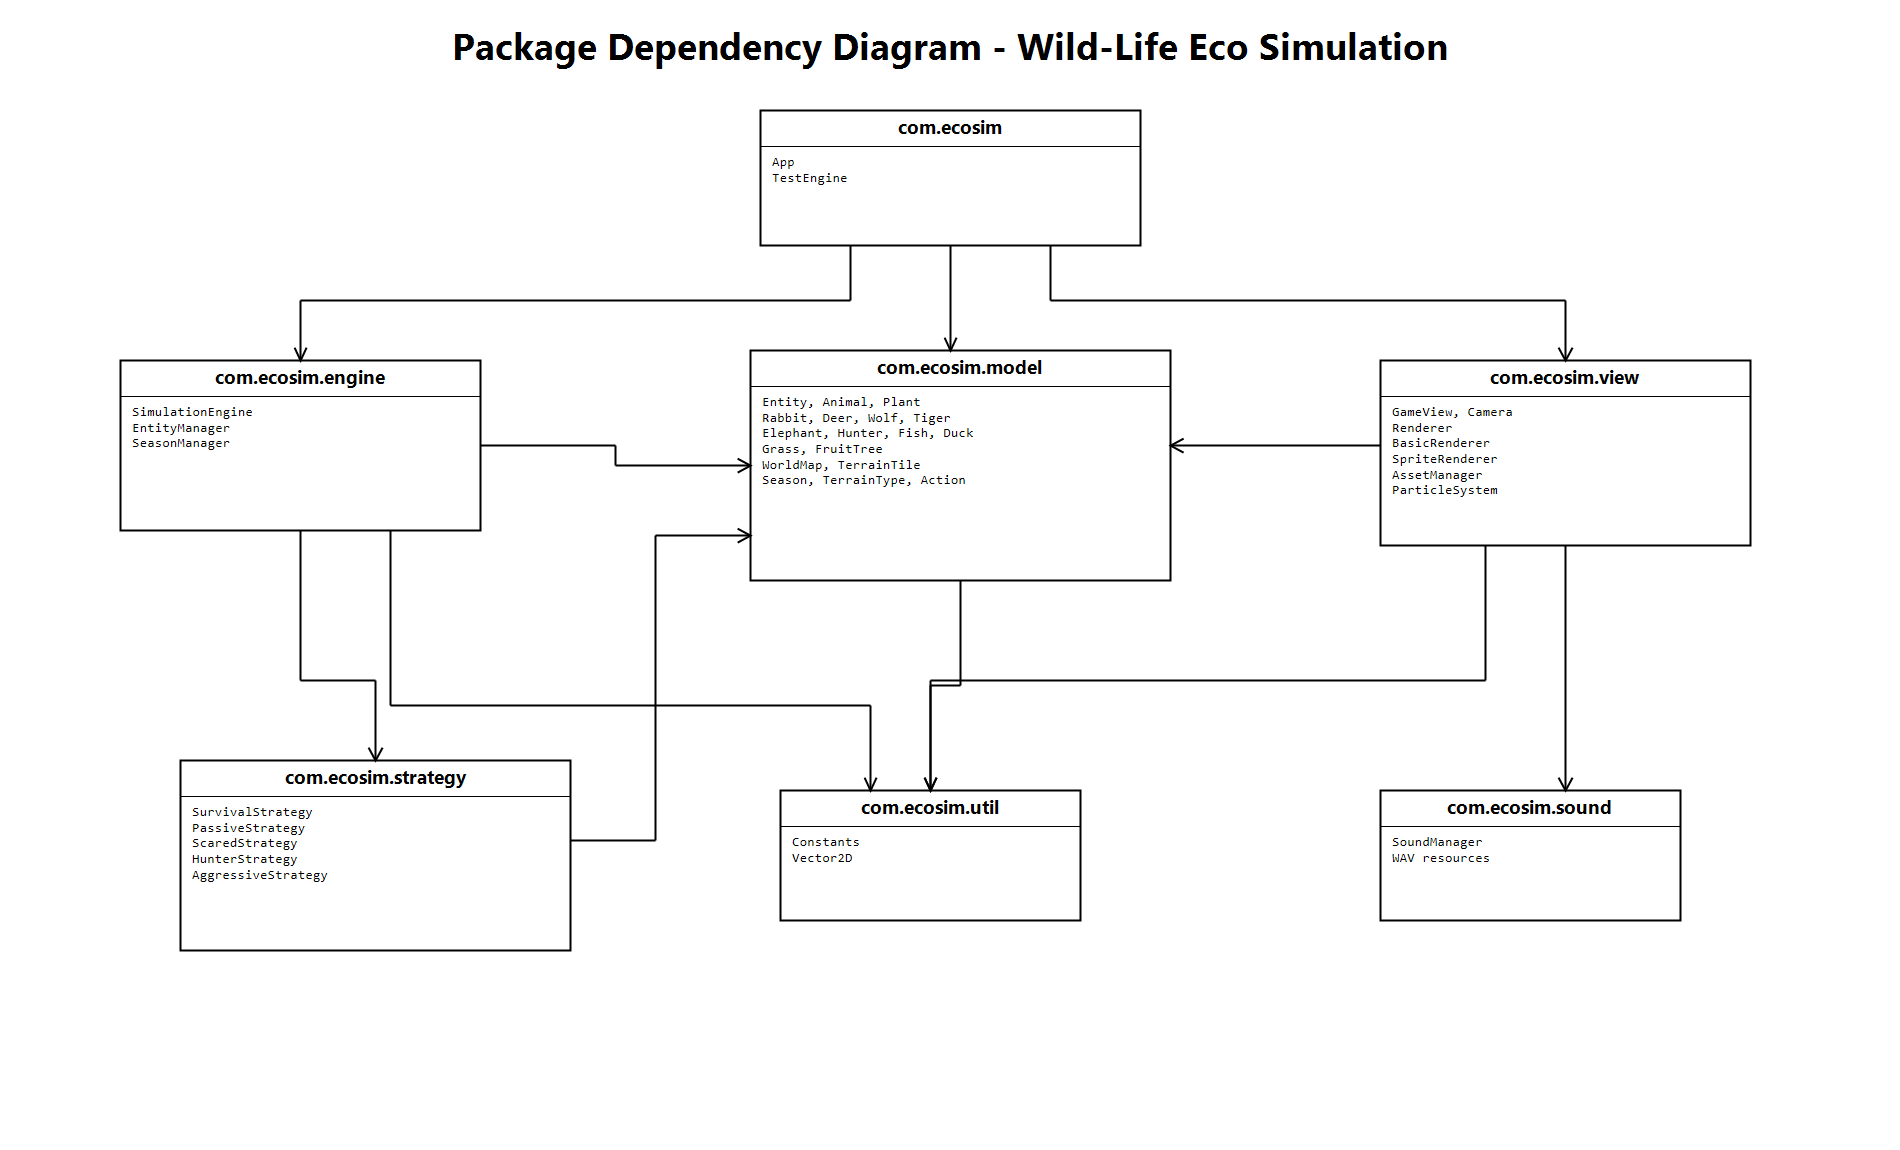
\includegraphics[width=0.95\textwidth]{uml/package-diagram.png}
    \caption{So do cac package trong project}
\end{figure}

\begin{table}[H]
    \centering
    \caption{Mo ta cac package trong project}
    \begin{tabular}{|c|p{4cm}|p{8cm}|}
        \hline
        \textbf{STT} & \textbf{Package} & \textbf{Vai tro} \\
        \hline
        1 & \texttt{com.ecosim} & Chua lop khoi dong ung dung \texttt{App} va lop \texttt{TestEngine}. \\
        \hline
        2 & \texttt{com.ecosim.model} & Chua cac lop mo hinh du lieu va logic sinh hoc: thuc the, dong vat, thuc vat, ban do, dia hinh, mua va hanh dong. \\
        \hline
        3 & \texttt{com.ecosim.engine} & Chua logic dieu khien mo phong: vong lap tick, quan ly thuc the, quan ly mua, sinh san, don dep, uong nuoc va xu ly va cham. \\
        \hline
        4 & \texttt{com.ecosim.strategy} & Chua cac chien luoc hanh vi cua dong vat theo Strategy Pattern. \\
        \hline
        5 & \texttt{com.ecosim.view} & Chua giao dien JavaFX, canvas, camera, renderer, sprite va hieu ung hat. \\
        \hline
        6 & \texttt{com.ecosim.sound} & Chua \texttt{SoundManager} de quan ly va phat am thanh theo su kien. \\
        \hline
        7 & \texttt{com.ecosim.util} & Chua cac tien ich dung chung nhu \texttt{Constants} va \texttt{Vector2D}. \\
        \hline
    \end{tabular}
\end{table}

\subsection{Cac lop chinh}

\begin{figure}[H]
    \centering
    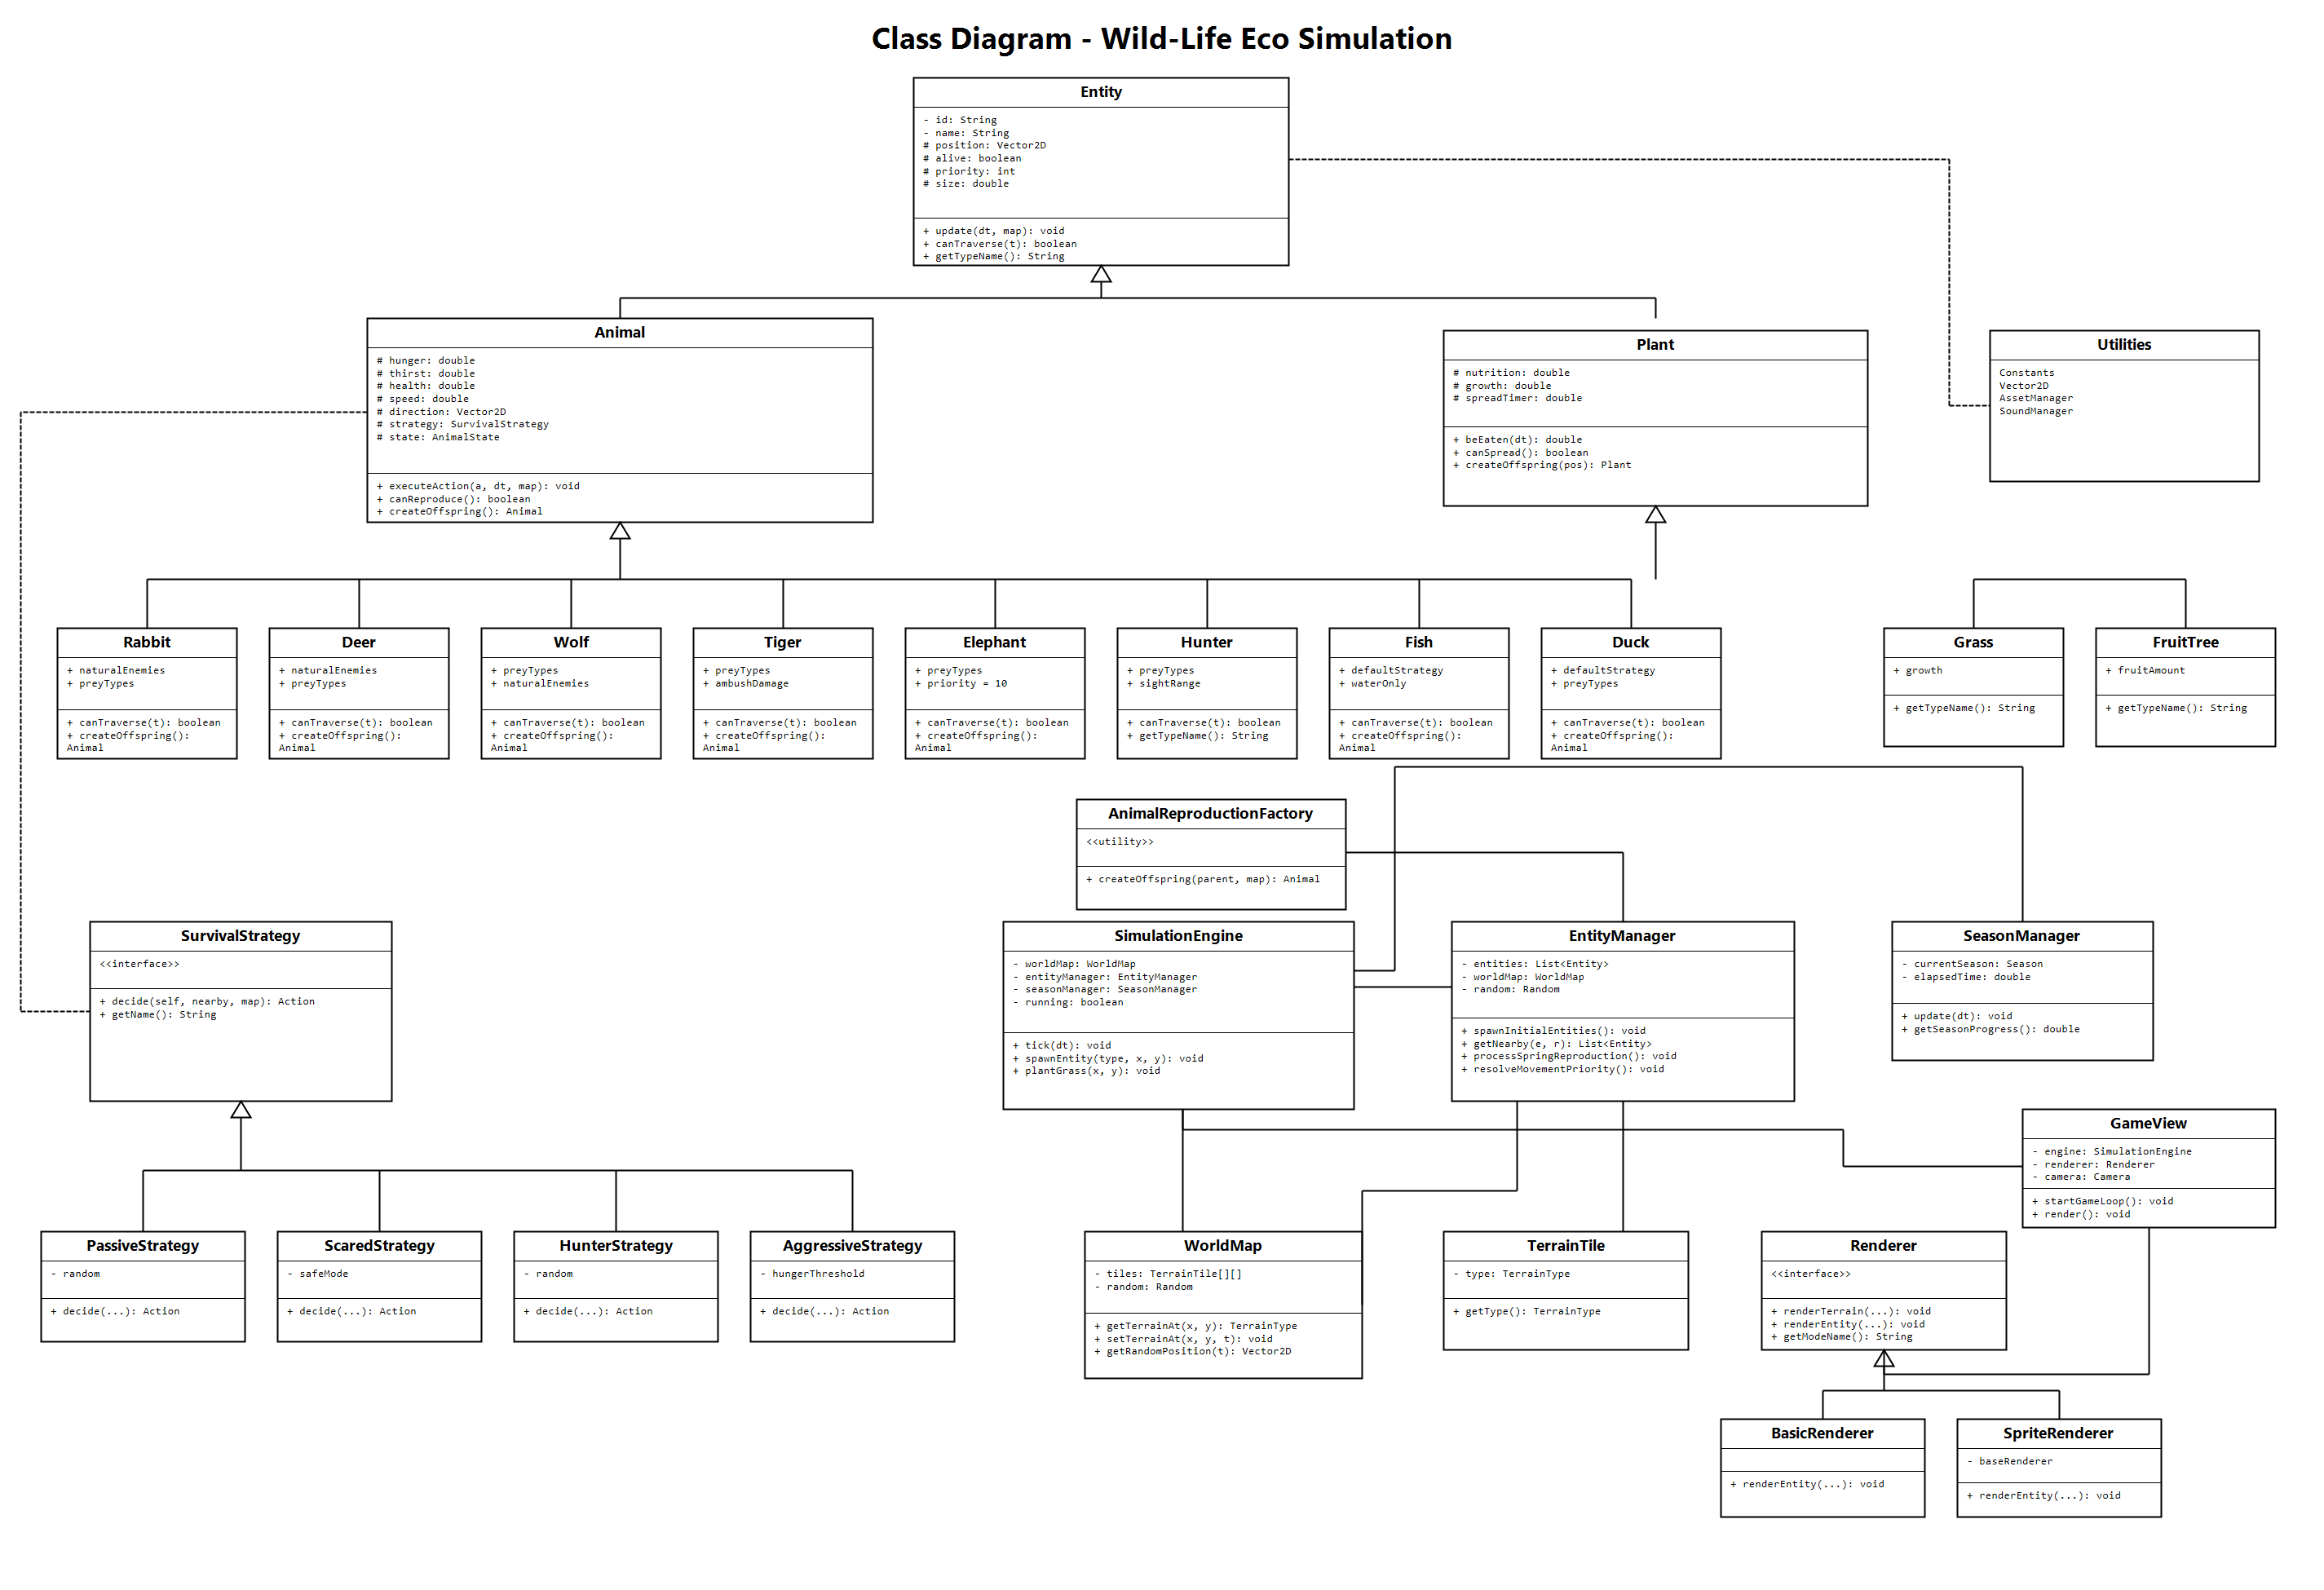
\includegraphics[width=0.95\textwidth]{uml/class-diagram.png}
    \caption{So do cac lop chinh trong project}
\end{figure}

\begin{longtable}{|c|p{4cm}|p{8cm}|}
    \hline
    \textbf{STT} & \textbf{Lop} & \textbf{Mo ta} \\
    \hline
    1 & \texttt{App} & Entry point cua JavaFX, tao \texttt{SimulationEngine}, \texttt{GameView}, scene va load CSS. \\
    \hline
    2 & \texttt{SimulationEngine} & Dieu khien moi tick cua mo phong: cap nhat mua, entity, strategy, va cham, uong nuoc, doi strategy va cleanup. \\
    \hline
    3 & \texttt{EntityManager} & Quan ly danh sach entity, spawn ban dau, duy tri quan the, sinh san mua xuan, xu ly nuoc va thong ke so luong. \\
    \hline
    4 & \texttt{WorldMap} & Quan ly ban do 120 x 80 tile, sinh dia hinh va tim vi tri theo terrain. \\
    \hline
    5 & \texttt{Entity} & Lop cha truu tuong cho moi thuc the, gom id, ten, vi tri, trang thai song, priority va size. \\
    \hline
    6 & \texttt{Animal} & Lop cha truu tuong cho dong vat, quan ly hunger, thirst, health, speed, state, strategy, con moi va ke thu. \\
    \hline
    7 & \texttt{Plant} & Lop cha truu tuong cho thuc vat, quan ly tang truong, bi an va lan rong. \\
    \hline
    8 & \texttt{Rabbit}, \texttt{Deer} & Dong vat an thuc vat, co ke thu tu nhien va co the doi sang \texttt{AggressiveStrategy} khi qua doi. \\
    \hline
    9 & \texttt{Wolf}, \texttt{Tiger}, \texttt{Hunter} & Cac thuc the san moi, dung \texttt{HunterStrategy} de tim va duoi theo con moi. \\
    \hline
    10 & \texttt{Elephant} & Dong vat uu tien cao, an thuc vat, khong co ke thu tu nhien trong cau hinh hien tai. \\
    \hline
    11 & \texttt{Fish}, \texttt{Duck} & Cac sinh vat song chu yeu o nuoc hoac bun. \\
    \hline
    12 & \texttt{Grass}, \texttt{FruitTree} & Thuc vat co kha nang tang truong, bi an va tao them thuc vat moi. \\
    \hline
    13 & \texttt{SurvivalStrategy} & Interface quy dinh phuong thuc \texttt{decide()} cho hanh vi cua dong vat. \\
    \hline
    14 & \texttt{PassiveStrategy}, \texttt{ScaredStrategy}, \texttt{HunterStrategy}, \texttt{AggressiveStrategy} & Cac cai dat cu the cho hanh vi thu dong, so hai, san moi va lieu linh. \\
    \hline
    15 & \texttt{GameView} & Man hinh chinh, chua canvas, toolbar, sidebar thong ke, menu them entity va game loop JavaFX. \\
    \hline
    16 & \texttt{Renderer}, \texttt{BasicRenderer}, \texttt{SpriteRenderer} & Interface va hai che do ve: hinh co ban va sprite. \\
    \hline
    17 & \texttt{Camera} & Ho tro zoom, pan va chuyen doi toa do man hinh/toa do the gioi. \\
    \hline
    18 & \texttt{SoundManager} & Phat am thanh theo su kien nhu ho gam, soi tru, uong nuoc, an va buoc chan. \\
    \hline
    19 & \texttt{Vector2D} & Lop tien ich tinh toan toa do, vector, khoang cach, huong va noi suy. \\
    \hline
    20 & \texttt{Constants} & Chua cac hang so cau hinh: kich thuoc ban do, toc do, tam nhin, priority, gioi han quan the. \\
    \hline
\end{longtable}

\section{Cac ky thuat lap trinh huong doi tuong da ap dung}

\begin{longtable}{|c|p{3.2cm}|p{5cm}|p{5cm}|}
    \hline
    \textbf{STT} & \textbf{Ky thuat} & \textbf{Ap dung o dau} & \textbf{Loi ich} \\
    \hline
    1 & Dong goi & Cac thuoc tinh trong \texttt{Entity}, \texttt{Animal}, \texttt{Plant}, \texttt{WorldMap}, \texttt{EntityManager} duoc khai bao \texttt{private} hoac \texttt{protected}, truy cap qua getter/setter. & Bao ve trang thai noi bo, tranh sua truc tiep gay loi va giup kiem soat gia tri nhu hunger, thirst. \\
    \hline
    2 & Ke thua & \texttt{Animal} va \texttt{Plant} ke thua \texttt{Entity}; \texttt{Rabbit}, \texttt{Deer}, \texttt{Wolf}, \texttt{Tiger}, \texttt{Elephant}, \texttt{Hunter}, \texttt{Fish}, \texttt{Duck} ke thua \texttt{Animal}. & Tai su dung code chung ve vi tri, trang thai, nhu cau sinh ton, di chuyen va xu ly hanh dong. \\
    \hline
    3 & Da hinh & \texttt{SimulationEngine} xu ly danh sach \texttt{Entity}; khi gap \texttt{Animal} thi goi \texttt{strategy.decide()}; \texttt{Renderer} co hai cai dat \texttt{BasicRenderer} va \texttt{SpriteRenderer}. & Cho phep them loai entity, strategy hoac renderer moi ma khong can thay doi nhieu code dieu khien. \\
    \hline
    4 & Truu tuong hoa & \texttt{Entity}, \texttt{Animal}, \texttt{Plant} la abstract class; \texttt{SurvivalStrategy} va \texttt{Renderer} la interface. & An chi tiet cai dat, tap trung vao hanh vi can co cua moi nhom doi tuong. \\
    \hline
    5 & Strategy Pattern & \texttt{SurvivalStrategy} duoc cai dat boi \texttt{PassiveStrategy}, \texttt{ScaredStrategy}, \texttt{HunterStrategy}, \texttt{AggressiveStrategy}. & Tach logic hanh vi khoi lop dong vat, giup doi chien luoc runtime khi dong vat doi, gap nguy hiem hoac di san moi. \\
    \hline
    6 & Factory & \texttt{AnimalReproductionFactory.createOffspring()} tao con non theo tung loai. & Tap trung logic sinh san vao mot noi, de mo rong va de kiem soat vi tri spawn hop le. \\
    \hline
    7 & MVC / tach trach nhiem & \texttt{model} chua BioLogic, \texttt{engine} dieu khien simulation, \texttt{view} hien thi JavaFX. & Lam code de doc, de test va han che phu thuoc giua logic mo phong voi giao dien. \\
    \hline
    8 & Singleton don gian & \texttt{AssetManager.getInstance()} quan ly cache anh sprite. & Tai lai tai nguyen dung chung de tiet kiem bo nho va tranh lap code load anh. \\
    \hline
\end{longtable}

\section{Cong nghe su dung va thuat toan}

\subsection{Cong nghe su dung}

\begin{itemize}
    \item \textbf{Ngon ngu lap trinh:} Java 21.
    \item \textbf{Framework giao dien:} JavaFX 21, gom \texttt{javafx-controls}, \texttt{javafx-fxml}, \texttt{javafx-media}.
    \item \textbf{Cong cu build:} Maven, Maven Wrapper, JavaFX Maven Plugin.
    \item \textbf{Kiem thu:} JUnit Jupiter 5.10.2, Maven Surefire Plugin.
    \item \textbf{Tai nguyen:} CSS, anh sprite PNG, am thanh WAV.
    \item \textbf{Co so du lieu:} Project co khai bao PostgreSQL JDBC Driver trong \texttt{pom.xml}; tuy nhien phan code hien tai chua thay lop repository/database su dung truc tiep driver nay.
\end{itemize}

\subsection{Thuat toan va ky thuat xu ly noi bat}

\begin{itemize}
    \item \textbf{Vong lap simulation theo tick:} \texttt{SimulationEngine.tick()} cap nhat moi thuc the theo \texttt{deltaTime} va he so toc do.
    \item \textbf{Tim entity gan trong tam nhin:} \texttt{EntityManager.getNearby()} loc cac entity song co khoang cach nho hon tam nhin cua dong vat.
    \item \textbf{He thong hanh vi theo strategy:} moi dong vat nhan danh sach thuc the gan do va ban do, sau do strategy tra ve \texttt{Action}.
    \item \textbf{Di chuyen co gia toc va giam toc:} \texttt{Animal.doMoveTo()} tinh toc do theo terrain, giam toc khi gan muc tieu va dung noi suy vector de xoay huong muot hon.
    \item \textbf{Xu ly va cham mem:} \texttt{EntityManager.resolveMovementPriority()} day nhe entity uu tien thap ra xa entity uu tien cao.
    \item \textbf{Sinh dia hinh va tim vi tri hop le:} \texttt{WorldMap} quan ly tile va tim vi tri ngau nhien theo loai terrain.
    \item \textbf{Sinh san theo mua:} dau mua xuan, \texttt{EntityManager.processSpringReproduction()} tao con non theo xac suat va gioi han quan the.
    \item \textbf{Cache tai nguyen:} \texttt{AssetManager} tai sprite va cache de renderer su dung lai.
\end{itemize}

\section{Huong dan su dung chuong trinh}

\subsection{Cach chay chuong trinh}

\begin{enumerate}
    \item Cai dat Java 21 tro len.
    \item Mo thu muc project trong VS Code, IntelliJ IDEA, Eclipse hoac chay truc tiep bang terminal.
    \item Chay nhanh bang lenh:
    \begin{verbatim}
.\run.bat
    \end{verbatim}
    \item Hoac chay truc tiep bang Maven Wrapper:
    \begin{verbatim}
.\mvnw.cmd clean javafx:run
    \end{verbatim}
    \item De build va chay test:
    \begin{verbatim}
.\mvnw.cmd package
.\mvnw.cmd test
    \end{verbatim}
\end{enumerate}

\subsection{Cac thao tac chinh}

\begin{itemize}
    \item Nut \textbf{Bat dau/Tam dung}: chay hoac dung mo phong.
    \item Muc \textbf{Toc do}: thay doi toc do mo phong tu 0.5x den 8x.
    \item Nut \textbf{Do hoa}: doi giua che do Basic Shapes va Sprites.
    \item Muc \textbf{Xem vung}: chuyen nhanh camera den toan ban do, dong co, rung ram hoac ho nuoc.
    \item Click trai voi cong cu \textbf{Chon}: chon entity de xem trang thai nhu mau, do doi, do khat, strategy va vi tri.
    \item Click trai voi cong cu \textbf{Gieo co}, \textbf{Dat da}, \textbf{Dat bui ram}: them doi tuong vao ban do.
    \item Click phai tren ban do: mo menu them tho, huou, soi, ho, voi, tho san, ca, vit, co hoac cay an qua.
    \item Scroll chuot de zoom; keo chuot giua hoac dung cong cu \textbf{Chon} de pan camera.
\end{itemize}

\subsection{Mot so anh demo chuong trinh}

Project hien tai chua co san anh chup man hinh demo trong thu muc tai nguyen. Sau khi chay ung dung, nhom nen chup cac man hinh quan trong va dat vao thu muc \texttt{images}. Cac lenh chen anh mau:

\demoimage{images/demo-main.png}{Anh man hinh chinh sau khi chay \texttt{run.bat}.}{Man hinh chinh cua chuong trinh}

\demoimage{images/demo-sprite-mode.png}{Anh khi bat che do hien thi sprite.}{Che do hien thi sprite}

\demoimage{images/demo-selected-entity.png}{Anh sidebar khi chon mot entity tren ban do.}{Bang thong tin khi chon mot entity}

\section{Kiem thu}

Project co su dung JUnit Jupiter de kiem thu mot so hanh vi quan trong:

\begin{itemize}
    \item \texttt{HunterStrategyTest}: kiem tra chien luoc san moi di den nguon thuc an gan nhat va giu dung target khi duoi con moi.
    \item \texttt{TigerTest}: kiem tra sat thuong phuc kich cua ho khi tan cong trong rung va kha nang tho an nap trong bui ram trong khi soi khong vao duoc.
    \item \texttt{EntityManagerTest}: kiem tra huou doi sang \texttt{AggressiveStrategy} khi do doi xuong duoi nguong nguy hiem.
\end{itemize}

\section{Ket luan}

Nhom da xay dung duoc ung dung mo phong he sinh thai hoang da bang JavaFX theo huong lap trinh huong doi tuong. Chuong trinh the hien ro cac nguyen ly OOP thong qua he thong lop ke thua, interface, da hinh, dong goi va truu tuong hoa. Ngoai ra, project con ap dung Strategy Pattern de tach hanh vi dong vat, Factory de tao con non va tach biet logic mo phong voi giao dien.

\subsection{Han che}

\begin{itemize}
    \item Phan co so du lieu moi duoc khai bao dependency PostgreSQL, chua co lop repository/database su dung thuc te.
    \item Anh demo chua duoc luu san trong project.
    \item Mot so loai sinh vat nhu ca va vit chua co sprite PNG rieng trong thu muc tai nguyen, co the can bo sung de hien thi dep hon.
    \item Test moi tap trung vao mot so hanh vi chinh, chua bao phu het vong doi simulation.
\end{itemize}

\subsection{Huong phat trien}

\begin{itemize}
    \item Bo sung co so du lieu de luu lich su mo phong, cau hinh ban do va ket qua thong ke.
    \item Them man hinh cau hinh truoc khi bat dau mo phong.
    \item Bo sung nhieu loai dong vat, thuc vat, dia hinh va rule sinh thai moi.
    \item Mo rong test cho \texttt{WorldMap}, \texttt{SimulationEngine}, sinh san va xu ly va cham.
    \item Tao anh demo va bieu do UML bang cong cu nhu StarUML, PlantUML hoac Visual Paradigm de bao cao truc quan hon.
\end{itemize}

\section{Tai lieu tham khao}

\begin{enumerate}
    \item README cua project \texttt{Wild-Life Eco Simulation}.
    \item Tai lieu Java: \url{https://docs.oracle.com/en/java/}
    \item Tai lieu JavaFX: \url{https://openjfx.io/}
    \item Tai lieu Maven: \url{https://maven.apache.org/}
    \item Tai lieu JUnit 5: \url{https://junit.org/junit5/}
    \item Tai lieu UML: \url{https://www.uml.org/}
\end{enumerate}

\end{document}
